\section{Problem Formulation}
\label{sec:problem}

The input traffic estimation data can be viewed as a matrix, as shown
in Figure~\ref{fig:problem-as-matrix}. Each row represents an
advertisement and each column represents a keyword. If a keyword $i$
is already associated with advertisement $u$, then we have some
observed traffic value $\beta_{ui}$. Otherwise, no value is observed
(noted as $X$).

\textcolor{red}{ ADD THE MEASUREMENT METRIX HERE: precision?  Given
  the input traffic estimation matrix $M$, the goal for our model is
  to predict the value of unobserved items $X$. We measure the overall
  precision of prediction using the formula (???)  Our goal is to
  maximiz the prediction accuracy in Eq ()?  }

\textcolor{red}{ change the matrix figure as follows: make the X as
  red highlighted}
\begin{figure}[!ht]
  \centering
  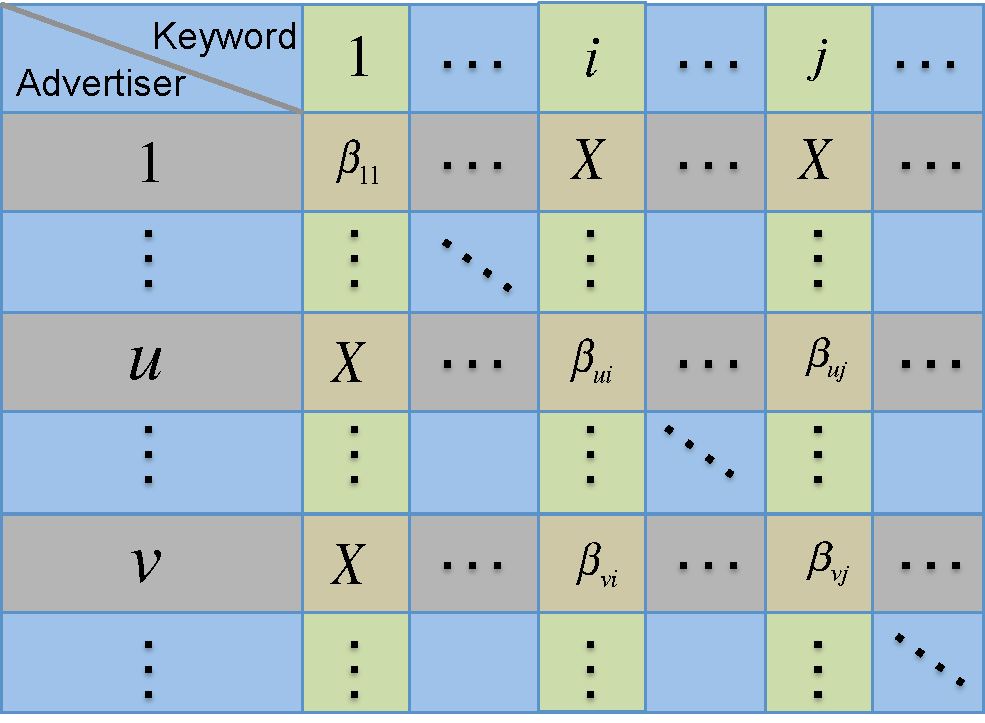
\includegraphics[width=0.35\textwidth]{figures/matrix.pdf}
  \caption{Matrix ??}
  \label{fig:problem-as-matrix}
\end{figure}

We approach this problem by mining the homogeneous similartiy across
advertisement and keyword dimentions, in another word, similarity
ratio of different keywords between similar advertisement should be
close to each other.  Instead of using only item-based or user-based
method, it is a synthetic multi-dimension model, which evaluates the
similarity cross item and user dimensions. Also, different from
item-based or user-based method, which uses a predefine static
similarity function and calculate the global optimal similarity, we
are using a local optimal function, which can dynamic involving
similarity using learned parameters, hence can support large scale
data in an efficient computation cost.
